\documentclass[a4paper,12pt]{article}
\usepackage{graphicx}

%opening
\title{\textbf{Studio di un modello di influenza culturale}}
\author{Jacopo Baldassarri (Corso di Laurea Magistrale in Informatica) \\Andrea Blasco (Dottorato in Economia) \\Elisa Omodei (Corso di Laurea Magistrale in Fisca)}

\begin{document}

\maketitle

\begin{abstract}
\end{abstract}

\clearpage
\section{Introduzione}
La domanda con cui esordisce R.~Axelrod nel suo articolo del 1997 \cite{Axelrod} \`{e}: \textquotedblleft If people tend to become 
more alike in their beliefs, attitudes, and behavior when they interact, why do not all such differences eventually disappear?\textquotedblright .
\\Il modello da lui proposto parte dal fatto che le persone diventano pi\`{u} simili quando interagiscono, ma spiega anche perch\`{e}
questa tendenza alla convergenza si ferma prima di arrivare ad una completa convergenza.
\\Il termine pi\`{u} generico per denotare le cose in cui le persone si influenzano a vicenda \`{e} \textit{cultura}.
Dunque questo termine verr\`{a} d'ora in poi utilizzato per indicare l'insieme di caratteristiche individuali che sono soggette all'influenza sociale.
\\Il modello di influenza sociale proposto astrae il principio fondamentale che il trasferimento di idee avviene pi\`{u} frequentemente
tra individui che sono gi\`{a} simili in alcuni aspetti, per affermare che la comunicazione \`{e} pi\`{u} efficace tra persone simili:
la probabilit\`{a} che un tratto culturale venga trasmesso da un individuo (o un gruppo) ad un altro dipende da quante altre caratteristiche
hanno gi\`{a} in comune.
\\Si parte dall'assunzione che la cultura deve soddisfare due semplici principi: 
\begin{itemize}
\item \`{e} pi\`{u} probabile che le persone interagiscano con altre persone con cui hanno gi\`{a} delle caratteristiche in comune,
\item le interazioni tra due persone tendono ad aumentare il numero di caratteristiche in comune.
\end{itemize}
Il modello assume che la cultura di un individuo si possa descrivere in termini di caratteristiche come la lingua, la religione,
l'abbigliamento, ecc. La cultura \`{e} dunque descritta come un insieme di caratteristiche. 
Per ogni caratteristica c'\`{e} un insieme di tratti, che sono i valori alternativi che una caratteristica pu\`{o} assumere.
Due individui hanno la stessa cultura se hanno gli stessi tratti per ognuna delle caratteristiche. 
Questa formulazione permette di definire il grado di somiglianza culturale tra due individui come la percentuale di caratteristiche che hanno lo stesso tratto.

\clearpage
\section{Il Modello di Axelrod}
Il modello di Axelrod \`{e} definito su un reticolo quadrato di dimensione lineare \textit{L}. 
Ogni sito \`{e} caratterizzato da un vettore \textit{F}-dimensionale di variabili $\sigma_f(i)$ che definiscono le caratteristiche culturali degli individui di quel sito.
Ogni caratteristica $f=1,\dots,F$ di ogni sito \`{e} inizialmente presa da una distribuzione casuale uniforme di interi compresi tra 0 e $q-1$: $\sigma_f = 0,1,\dots,q-1$.
Il parametro \textit{q} \`{e} una misura della variet\`{a} culturale (disordine) iniziale nel sistema.
Ad ogni passo temporale, una coppia di siti vicini \textit{i} e \textit{j} viene selezionata in modo casuale e viene calcolata la loro somiglianza culturale, cio\`{e} la quantit\`{a}:
\begin{equation}
 \omega_{i,j} = \frac{1}{F} \sum_{f=1}^F \delta_{\sigma_f(i) \sigma_f(j)}
\end{equation}
dove $d_{i,j}$ \`{e} la delta di Kronecker.
Con probabilit\`{a} $\omega_{i,j}$ avviene l'interazione: one delle caratteristiche per cui i tratti sono diversi 
$[ \sigma_f(i) \neq \sigma_f(j) ]$ viene selezionata e il tratto di \textit{j} viene posto uguale a quello di \textit{i}.
Con probabilit\`{a} $1-\omega_{i,j}$ non succede niente.
Uno \textit{sweep} di tutto il reticolo, cio\`{e} $L^2$ passi temporali, definisce l'unit\`{a} temporale.
Se tutte le caratteristiche sono uguali su un legame o se sono tutte diverse, nessun cambiamento pu\`{o} pi\`{u} avvenire sul tale legame.
Una tale configurazione \`{e} detta \textit{stato assorbente}. La dinamica si ferma quando un tale stato \`{e} raggiunto.
\\L'evoluzione dinamica \`{e} caratterizzata dalla competizione tra il disordine della configurazione iniziale e la spinta all'ordine
dovuta alle interazioni sociali locali. 
Quando $q$ \`{e} piccolo lo stato iniziale \`{e} quasi completamente uniforme, mentre quando $q$ \`{e} grande quasi tutti i siti
hanno caratteristiche $\sigma_f(i)$ completamente diverse dai propri vicini. Nei due casi ci aspettiamo che il sistema converga ad
uno stato uniforme o altamente fragmentato in cui dominano le interazioni o il disordine, rispettivamente.
Castellano \textit{et al.} \cite{Castellano} hanno studiato come queste due situazioni limite sono connesse al variare di $q$
e hanno trovato che per $F>2$ avviene una transizione netta ad un certo valore critico $q_c$ di $q$ caratterizzata da un
improvviso calo del parametro d'ordine $<S_{max}>/L^2$, transizione che diventa sempre pi\`{u} ripida all'aumentare di $L$.
Ci\`{o} mette in evidenza una transizione tra una fase culturalmente polarizzata per $q<q_c$, dove una delle regioni culturali ha
le dimensioni dell'ordine di tutto il sistema, e una fase culturalmente frammentata, dove tutte le regioni culturali hanno dimensione finita.
La situazione \`{e} invece diversa per $F=2$, per cui la frazione occupata da $<S_{max}>/L^2$ diminuisce con continuit\`{a} all'aumentare di $q$.
Castellano ha inoltre trovato che la distribuzione delle dimensioni delle regioni culturali $P_L(s,q)$ per valori di $q$ attorno alla transizione
segue una legge di potenza $P_L(s,q) = s^{-\tau}$.

\subsection{Risultati Numerici}
Abbiamo dunque iniziato il nostro studio effettuando delle simulazioni numeriche del modello di Axelrod nel caso $F=3$ e $L=20$.
Abbiamo scelto il caso $F=3$ per poter avere una buona visualizzazione grafica del modello. Infatti in questo modo ci \`{e} possibile
associare ad ogni caratteristica una componente RGB e possiamo dunque rappresentare ogni cultura con un colore attraverso una
corrispondenza biunivoca.
La Figura \ref{transiz_ret} mostra la transizione, ovvero come varia il parametro d'ordine $<S_{max}>/L^2$ al variare di $q$. 
Possiamo osservare una transizione abbastanza netta attorno a $q = q_c \simeq 12$. I valori sono mediati su dieci realizzazioni, 
per cui \`{e} riportata anche la varianza.
La Figura \ref{cum_distr_size_ret} mostra la distribuzione, in scala logaritmica, delle dimensioni delle regioni culturali 
per $q_c = 12$. Possiamo osservare che essa sembra seguire effettivamente una legge di potenza con esponente $\tau \simeq 2$.

\begin{figure}[!ht]
\begin{center}
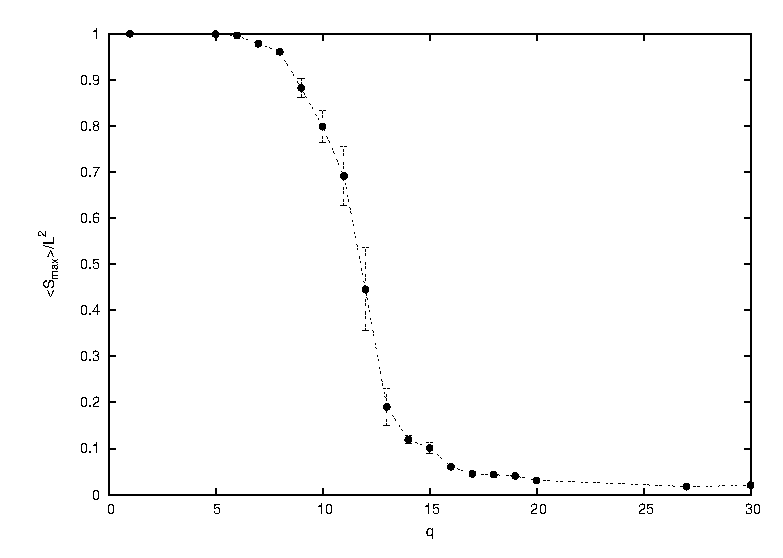
\includegraphics[width=\textwidth]{transizione_ret.eps}
\end{center}
\caption{Transizione tra una fase culturalmente polarizzata e una fase culturalmente fragmentata al variare di $q$ nel caso del modello di Axelrod originale, ovvero su reticolo con quattro vicini. La transizione \`{e} studiata attraverso il parametro d'ordine $<S_{max}>/L^2$. I risultati ottenuti sono mediati su dieci realizzazioni.}
\label{transiz_ret}
\end{figure}

\begin{figure}[!ht]
\begin{center}
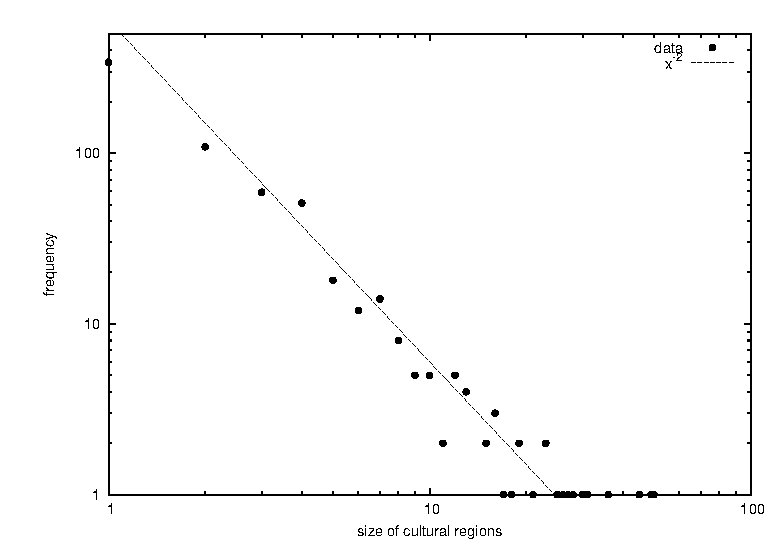
\includegraphics[width=\textwidth]{cum_distr_size_ret.eps}
\end{center}
\caption{Distribuzione delle dimensioni delle regioni culturali per $q = q_c$, in scala logaritmica per entrambi gli assi, nel caso del modello di Axelrod originale, ovvero su reticolo con quattro vicini. I risultati ottenuti sono basati su dieci realizzazioni.}
\label{cum_distr_size_ret}
\end{figure}

\clearpage

\section{Applicazione del Modello di Axelrod allo Small World di Kleinberg}
Abbiamo poi deciso di studiare una variazione del modello di Axelrod applicando la dinamica del modello ad un diverso tipo di network. Invece di utilizzare un reticolo, abbiamo utilizzato un particolare tipo di network proposto da Kleinberg in \cite{Kleinberg}.
\\ \\Partiamo da un insieme di $N$ nodi identificati da un insieme di punti su un quadrato di dimensioni $L \times L$, ${(i,j) : i \in {1,2,\dots,L}, j \in {1,2,\dot,L}}$ 
e definiamo la distanza tra due nodi $(i,j)$ e $(k,l)$ come $d((i,j),(k,l)) = \sqrt{(i-k)^2+(j-l)^2}$. 
Dato il parametro costante $p \geq 0$, ogni nodo $u$ \`{e} connesso attraverso un link diretto con ogni altro nodo che si trova a distanza $p$. Questi sono i suoi contatti locali.
Dati altri due parametri, $l \geq 0$ e $\delta \geq 0$, vengono costruiti anche link diretti da $u$ a $l$ altri nodi (contatti a lungo raggio), utilizzando tiri random indipendenti;
l'$i$-esimo link diretto da $u$ termina su $v$ con probabilit\`{a} proporzionale a $[d(u,v)]^{-\delta}$.
\\Questo modello ha una semplice interpretazione geografica: gli individui vivono su una griglia e conoscono i loro vicini per
un certo numero di passi in ogni direzione e hanno anche un certo numero di conoscenti distribuiti pi\`{u} ampiamente su tutta la griglia.
Vedendo $p$ e $l$ come costanti, otteniamo una famiglia ad un parametro di modelli di reti variando l'esponente $\delta$.
Quando $\delta = 0$ abbiamo una distribuzione uniforme dei contatti a lungo raggio, la stessa distribuzione utilizzata nel modello
di Watts e Strogatz - i contatti a lungo raggio sono scelti indipendentemente dalla loro posizione sulla griglia.
Al crescere di $\delta$, i contatti a lungo raggio di un nodo diventano sempre pi\`{u} clusterizzati nelle vicinanze del nodo stesso.
Dunque $\delta$ serve da parametro strutturale per misurare quanto ampiamente \`{e} interconnessa la societ\`{a} dei nodi.
\\ \\Abbiamo dunque creato dei network caratterizzati da $p=0$ e $l=4$, facendo variare il parametro $\delta$. In questo modo il caso del reticolo con 4 vicini si ottiene nel limite $\delta = \infty$.
\\ \\In questo caso il sistema non raggiunge mai uno stato \textit{completamente} assorbente a causa della direzionalit\`{a} dei link. 
Si possono infatti creare delle situazioni in cui un agente $i$ viene alternativamente influenzato da due suoi vicini che hanno in comune tra loro e con l'agente $i$ due caratteristiche su tre. Se i link fossero diretti tutti e tre gli agenti dopo un certo numero di step avrebbero le stesse features, ma se l'agente $i$ ha dei link uscenti verso questi altri due agenti ma non viceversa, allora i due agenti continueranno ad influenzare l'agente $i$, ma esso non potr\`{a} influenzare loro.
Comunque dopo un certo numero di step temporali tutte le quantit\`{a} interessanti del sistema rimangono costanti in media e il sistema \`{e} dunque termalizzato. In questo caso quindi la dinamica viene fermata dopo un numero di step temporali pari al quadrato del numero di agenti, tempo che abbiamo visto essere pi\`{u} che sufficiente per raggiungere la termalizzazione.
\\ \\Quello che abbiamo trovato \`{e} che al diminuire di $\delta$ la transizione dalla fase culturalmente polarizzata a quella culturalmente fragmentata avviene in modo sempre meno netto, com'\`{e} possibile osservare in Figura \ref{transiz}.
La pendenza della curva di transizione dipende dunque dalla geografia del network: pi\`{u} globalizzata \`{e} la rete, maggiore \`{e} il numero di possibili tratti necessari perch\`{e} vi sia una netta fragmentazione culturale.
\\Inoltre anche in questo caso otteniamo delle leggi di potenza per la distribuzione delle dimensioni delle regioni culturali attorno a $q_c$, con esponente $\tau$ che diminuisce al diminuire di $\delta$ (Figura \ref{cum_distr_size}).

\begin{figure}[!ht]
\begin{center}
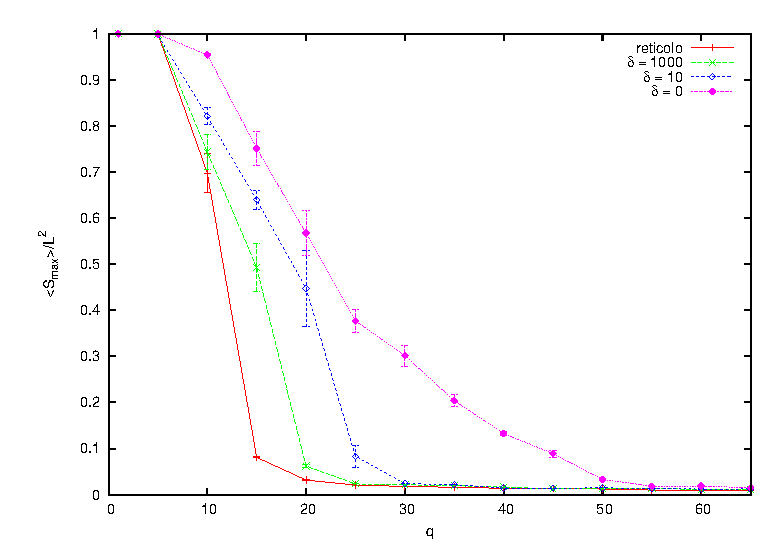
\includegraphics[width=\textwidth]{transizione.eps}
\end{center}
\caption{Transizione tra una fase culturalmente polarizzata e una fase culturalmente fragmentata al variare di $q$, per diversi valori del parametro $\delta$. La transizione \`{e} studiata attraverso il parametro d'ordine $<S_{max}>/L^2$. I risultati ottenuti sono mediati su dieci realizzazioni.}
\label{transiz}
\end{figure}

\begin{figure}[!ht]
\begin{center}
\includegraphics[width=\textwidth]{cum_distr_size_qCritico.eps}
\end{center}
\caption{Distribuzione delle dimensioni delle regioni culturali per $q = q_c$, in scala logaritmica per entrambi gli assi, per diversi valori del parametro $\delta$. I risultati ottenuti sono basati su dieci realizzazioni.}
\label{cum_distr_size}
\end{figure}

\clearpage
\section{Software}

\newpage
\begin{thebibliography}{10}
\normalsize
 \bibitem{Axelrod} R.~Axelrod, \textit{The Dissemination of Culture}, Journal of Conflict Resolution, 41, 203 (1997)
 \bibitem{Castellano} C.~Castellano, M.~Marsili and A.~Vespignani, \textit{Nonequilibrium phase transition in a model for social influence}, Phys.~Rev.~Lett. 85, (2000)
 \bibitem{Kleinberg} J.~Kleinberg, \textit{The Small-World Phenomenon: An Algorithmic Perspective}, Proceedings of the thirty-second annual ACM symposium on Theory of computing (2000)
\end{thebibliography}

\end{document}
